\section{Описание предметной области}

\subsection{Логическое и реляционное программирование}

{\bf Логическое программирование}~--- это вид декларативного программирования,
основанный на формальной логике. Программы представляются в виде
утверждений, представляющихся логическими формулами и описывающих
определённую область проблем.
``Вычисление'' программы в контексте логического программирования производится
в форме \emph{поиска} доказательства утверждений на основе заданных
фактов --- аксиом --- и правил вывода в соответствии с заданной
\emph{стратегией поиска}~\cite{logicMJ}.

Стратегия поиска задаёт,
каким образом происходит обход пространства поиска ответов, и,
как следствие, определяет как, какие и в каком порядке будут находиться
ответы. Стратегия поиска, при которой каждый возможный ответ будет со временем
выдан, называется \emph{полной}. Чаще применяются \emph{неполные} стратегии,
поскольку они менее требовательны к вычислительным ресурсам~\cite{currySearch}.

Самые известные языки логического программирования --- языки семейства Prolog.
Prolog применяется для доказательства теорем~\cite{prologTheorem},
проектирования баз знаний, создания экспертных систем~\cite{prologExSys}
и искусственного интеллекта~\cite{prologInt}.
Prolog строится на логике предикатов первого порядка в форме дизъюнктов
Хорна (то есть дизъюнктов только с одним положительным литералом) и
использует \emph{метод резолюций}, основанный на доказательстве от
противного, для решения задач.
Prolog вводит разнообразные синтаксические конструкции с
\emph{побочными эффектами}, то есть с действиями, приводящими к изменению
\emph{окружения} программы, к примеру, оперaтор отсечения~\origin{cut},
который влияет на способ вычисления программы, предотвращая нежелательные
вычисления.
Также он использует стратегию обхода в глубину, что приводит к тому, что
поиск может ``зациклиться'' и никогда не выдать оставшиеся решения,
но, тем не менее, благодаря своим расширениям Prolog
остаётся хорошим решением для задач из своей области применения~\cite{logicMJ}.

% Подобные операторы обычно используются для того, чтобы
% повысить эффективность программ, однако 

% Другие языки логического программровани, такие как Mercury\cite{mercury} или 
% Curry\cite{curry}, являются 

% {\bf Логическое программирование}~--- это вид декларативного программирования,
% основанный на логике предикатов первого порядка в форме дизъюнктов Хорна
% (то есть дизъюнктов
% с только одним положительным литералом),
% применяющий принципы логического вывода на основе заданных фактов и правил.
% Программа, написанная на логическом языке --- это множество логических формул,
% описывающих определённую область проблем.\cite{logicMJ}

% Существует множество языков логического программирования, таких как Prolog, Curry, Mercurry,
% однако самые известные --- языки семейства Prolog. Prolog применяется для доказательства
% теорем, проектирования баз знаний, создания экспертных систем и искусственного интеллекта.

% Prolog построен на \emph{методе резолюций}, который является обобщением метода
% ``доказательства от противного'', а в частности --- на \emph{линейном} методе
% резолюций \origin{Linear resolution with Selection function for Definition clauses}.
% При вычислении программы правило резолюции применяется не к случайных дизъюнктам,
% а в строго установленном порядке. В случае, когда вычисления дизъюнкта прошло
% неудачно, происходит \emph{откат} к прошлому состоянию программы, на котором
% выбирался неудавшийся дизъюнкт\cite{logicMJ}.
% 
% Помимо этого, Prolog вводит разнообразные синтаксические конструкции с побочными \emph{эффектами},
% то есть с действиями, приводящими к изменению \emph{окружения} программы,
% к примеру, оперaтор отсечения~\origin{cut},
% который влияет на способ вычисления программы.

% Это свойства определяют Prolog как язык, однако из-за них теряется свойство \emph{реляционности}.

% % 
% % Пример программы на Prolog приведён в Листинге~\ref{lst:memberProlog}.
% % 
% % \begin{lstlisting}[language=Prolog,caption={Проверка принадлежности элемента списку},captionpos=b,label={lst:memberProlog}]
% % member(X, [X | T]).
% % member(X, [H | T]) :- member(X, T).
% % \end{lstlisting}
% % 
% % В этой программе проверяется принадлежность элемента списку. Есть два возможных
% % варианта происходящего: либо элемент равен элементу в голове списка



{\bf Реляционное программирование}~--- это форма чистого логического
программирования, в которой программы задаются как набор
математических {\it отношений}~\cite{byrdMK}.
%Реляционное программирование ориентировано
%на получение \emph{значимых} ответов, как бы ни использовались отношения

Исторически, понятие реляционного программирования появилось
раньше~\cite{relML} и задавало саму концепцию программы как отношения,
когда логическое --- появилось позже и предоставляло реализацию его
идей~\cite{logicMJ}.
Однако в данной работе под реляционным программированием понимается
непосредственно то, что указано выше в определении.

В терминах реляционного программирования, к примеру, сложение $X + Y = Z$
может быть выражено отношением\footnote{Символ $\ ^o$ традиционно
используется для обозначения отношения.}
\[\text{add}^o (X, Y, Z),\]
которое в зависимости от того, какие переменные заданы, порождает
все возможные значения переменных, при которых отношение выполняется:
\begin{itemize}
\item \rel{add}(1, 2, 3) --- проверка, что значения находятся в отношении;
\item \rel{add}(1, 2, A) --- поиск всех таких A, при которых 1 + 2 = A;
\item \rel{add}(A, B, 3) --- поиск всех таких A и B, при которых A + B = 3;
\item \rel{add}(A, B, C) --- поиск всех троек A, B и С, при которых A + B = C.
\end{itemize}

Чистые отношения не предполагают функциональных зависимостей между переменными,
поэтому поиск можно проводить в разных ``направлениях'', в зависимости от
того, какие переменные заданы, как показано выше в примере.

%Когда же отношения вырождаются в функциональные и появляется
%явная зависимость между переменными, тогда можно говорить про запуск
Для функциональных отношений можно ввести понятие направления: для запуска
в ``прямом'' направлении задаются входные аргументы, а для запуска в
``обратном'' задаётся результат.

К примеру, отношение ``меньше'' для двух чисел X и Y можно задавать как
\rel{less}(X, Y) и получить чистое реляционное отношение.
Отношение же с функциональной зависимостью ---
\rel{$\text{less}_2$}(X, Y, R), где R сообщает, состоят ли X и Y
в отношении, и тогда задание X и Y будет
прямым направлением, а задание R --- обратным.

% Отличительная черта реляционного программирования в том, что с каким бы
% набором аргументов отношение ни было запущено, обязательно должны быть
% найдены все ответы, если они есть. Для сравнения, в Prolog 

% Ссылка на Булычева
Одно из применений реляционной парадигмы --- {\it реляционные интерпретаторы}.
Для языка $L$ его интерпретатор -- это функция $\text{eval}_L$, которая принимает
на вход программу $p_L$ на этом языке, её вход $i$ и возвращает некоторый выход $o$:
\[ \text{eval}_L (p_L, i) \equiv \llbracket p_L \rrbracket (i) = o \]
Реляционную версию интерпретатора можно представить как отношение:
\[ \text{eval}_L^o(p_L, i, o). \]

При запуске такого отношения в разных направлениях можно не только вычислять результат,
но и по программе $p_L$ и выходу $o$
искать возможные входы $i$ или вовсе генерировать программу по указанным
выходам и входам.
% решать задачи поиска по задаче распознавания~\cite{lozov},
%генерировать программы по заданной спецификации входа $i$ и выхода $o$~\cite{unifiedMK}.

Можно отметить, что в языках, основанных на классическом Prolog, производить
подобные вычисления для получения осмысленных результатов значительно труднее.
%для достижения адекватной производительности используются операторы
%отсечения, при которых код теряет реляционную гибкость.


\subsubsection{miniKanren}

% Byrd
{\it miniKanren} -- семейство встраиваемых предметно-ориентированных языков,
специально спроектированное для реляционного программирования~\cite{byrdMK}.

Основная реализация miniKanren написана на языке Scheme~\cite{reasonedSchemer},
однако существует множество реализаций в ряде других языков, в том числе
Clojure, OCaml, Haskell и другие\footnote{Официальный сайт языка miniKanren: \url{minikanren.org}, дата последнего посещения: 19.05.2020}.

miniKanren предоставляет набор базовых конструкций: унификация ($\equiv$),
конъюнкция $(\land)$, дизъюнкция $(\lor)$, введение свежей переменной
(\lstinline{fresh}), вызов реляционного отношения,
--- представляющий ядро языка, и разнообразные расширения, к примеру, оператор неэквивалентности
\origin{disequality constraint} или операторы, не являющиеся чистыми, к примеру, предоставляющие функциональность
отсечения из Prolog. Хотя в miniKanren введены операторы с эффектами,
его использование как реляционного языка подразумевает работу только с чистыми операторами.

Классический пример --- программа конкатенации двух списков --- указан
на рисунке~\ref{fig:appendo}.
Здесь список \lstinline{R} является конкатенацией списков \lstinline{X} и
\lstinline{Y} в случае, когда список \lstinline{X} пуст, а \lstinline{Y}
равен \lstinline{R}, либо когда \lstinline{X} и \lstinline{R} декомпозируются
на голову и хвост, а их хвосты состоят в отношении конкатенации с \lstinline{Y}.

\begin{figure}[h!]
\begin{lstlisting}[mathescape,language=Haskell,extendedchars=\true,frame=single,basicstyle=\ttfamily]
$\text{append}^o$ X Y R =
  X $\equiv$ [] $\land$ Y $\equiv$ R $\lor$
  fresh (H X' R')
    (X $\equiv$ H :: X') $\land$
    (R $\equiv$ H :: R') $\land$
    $\text{appendo}^o$ X' Y R'
\end{lstlisting}

\caption{Пример программы на miniKanren (\lstinline{::} --- конструктор списка)}
\label{fig:appendo}
\end{figure}

Для выполнения конкатенации над списками необходимо сформировать
\emph{запрос}~(или \emph{цель}).
В запросе в аргументах указываются либо замкнутые термы, либо термы
со свободными переменными. Результатом выполнения является список
подстановок для свободных переменных, при которых отношение выполняется;
когда свободных переменных нет, подстановка, соответственно, пустая.
Полное отсутствие каких-либо подстановок говорит об отрицательном результате
выполнения запроса.

На рисунке~\ref{fig:appendoExample} приведён пример запроса, в котором мы хотим
найти возможные значения переменных \lstinline{Y} и \lstinline{R}. Потенциально
может быть бесконечное число ответов, к примеру, когда все аргументы в запросе
--- переменные, поэтому в системах miniKanren есть возможность запрашивать
несколько первых ответов; в примере, это число 1. Ответы могут содержать в себе
как конкретные замкнутые термы (к примеру, числа), так и свободные переменные,
которые в примере обозначаются как $\text{\_.}_n$. В примере одна и также
свободная переменная $\text{\_.}_0$ назначена и \lstinline{Y}, и \lstinline{R}.
Это означает, что какое бы ни было значение \lstinline{Y}, оно всегда будет
являться хвостом хвоста \lstinline{R}.

\begin{figure}[h!]
\begin{lstlisting}[mathescape,language=Haskell,extendedchars=\true,frame=single,basicstyle=\ttfamily]
> run 1 (Y R) ($\text{append}^o$ [1, 2] Y R)
Y = $\text{\_.}_0$
R = 1 :: 2 :: $\text{\_.}_0$
\end{lstlisting}
\caption{Пример выполнения запроса к отношению конкатенации.}
\label{fig:appendoExample}
\end{figure}

В определение miniKanren входит особый алгоритм поиска ответов --- чередующийся
поиск \origin{interleaving search}, %основанный на поиске в глубину,
который рассматривает всё пространство поиска и является
полным~\cite{interleaving}.
% гарантирует, что если существует ответ, то алгоритм его предоставит за конечное время\cite{interleaving}.
%Для сравнения, обычный поиск в глубину, используемый в классическом Prolog при методе резолюций, может зациклиться
%или разойтись перед тем, как предоставить все ответы.
Это свойство чередующегося поиска определяет, вместе с отсутствием
нечистых расширений, реляционность miniKanren. 

% Применимость
Хотя miniKanren уже применяется в индустрии для поиска лечения редких
генетических заболеваний в точной медицине~\cite{medMK},
на данном этапе своего развития используется в основном в исследовательских
целях:
\begin{itemize}
\item реляционные интерпретаторы на miniKanren для решения задач поиска~\cite{lozov};
\item техника программирования по примерам~\cite{unifiedMK};
\item для доказательства теорем~\cite{mkProver} ;
\item в области вычислительной лингвистики~\cite{mkLing}.
\end{itemize}

%Одно из интересных применений miniKanren --- {\it реляционные интерпретаторы}.
%Для языка $L$ его интерпретатор -- это функция $\text{eval}_L$, которая принимает
%на вход программу $p_L$ на этом языке, её вход $i$ и возвращает некоторый выход $o$:
%\[ \text{eval}_L (p_L, i) \equiv \llbracket p_L \rrbracket (i) = o,\]
%где $\llbracket \bullet \rrbracket $ --- семантика языка L.
%Тогда в miniKanren интерпретатор описывается отношением $\text{eval}^o_L(p_L, i, o)$.
%При запуске такого отношения на разном наборе аргументов можно добиться интересных эффектов:
%\begin{itemize}
%\item по программе $p_L$ и выходу $o$ искать возможные входы $i$ (запуск программы в обратном направлении);
%  %: $\text{eval}^o(\text{add}, I, 3)$
%\item решать задачи поиска по задаче распознавания~\cite{lozov};
%\item генерировать программы по заданной спецификации входа $i$ и выхода $o$
%(техника программирования по примерам)\cite{unifiedMK}.
%\end{itemize}

% \todo{проблемы miniKanren: долгое вычисления сложных алгоритмов, долгие вычисления в обратном направлении.}
Однако miniKanren обладает рядом существенных недостатков. Несмотря на то,
что он ближе всего подошёл к реализации чистой реляционности, вычислительно
он всё же зависим от сложности и ветвистости программ, из-за чего их запуск в
разных направлениях может работать с разной скоростью, в особенности запуск в обратном направлении,
который зачастую работает очень медленно.
Также, описывать сложные задачи в качестве отношений --- нетривиальная задача,
наивно написанные реляционные программы вычисляются крайне неэффективно.
Из-за чего, к примеру, существует транслятор из функционального языка в
miniKanren~\cite{trconv}, однако порождаемые им отношения --- функциональные,
а запуск их в обратном направлении, как указывалось выше, крайне
непроизводителен~\cite{lozov}.

Одно из возможных решения проблем производительности --- специализация.


\subsection{Специализация программ}

{\bf Специализация} --- это метод автоматической оптимизации программ,
при котором из программы удаляются избыточные вычисления,
на основе информации о входных аргументах программы~\cite{jones}.

% Специализацию программ также называют \emph{частичными} или
% \emph{смешанными вычислениями}\cite{jones}.

{\it Специализатор} $\text{spec}_L$ языка $L$ принимает на вход программу $p_L$ и часть известного входа этой
программы $i_s$ (\emph{статические} данные) и генерирует новую программу $\hat{p}_L$, которая ведёт себя на оставшемся
входе $i_d$ (\emph{динамические} данные) также, как и оригинальная программа (формула~\ref{eq:spec}).

\begin{equation}
  \llbracket \text{spec}_L(p_L, i_s) \rrbracket (i_d) \equiv \hat{p}_L (i_d) \equiv \llbracket p_L \rrbracket (i_s, i_d)
\label{eq:spec}
\end{equation}

% Эффекты специализаторов
Специализатор производит все вычисления, зависимые от статических данных,
протягивание констант, инлайнгинг и другие.

Одно из интересных теоретических применений специализации --- это
\emph{проекции Футамуры}~\cite{futamura}. Процесс специализации интерпретатора
на программу на языке $L$ $\text{spec}_L(\text{eval}_L, p_L)$
порождает \emph{скомплированную} программу $\hat{p}_L$, а процесс специализации
специализатора на интерпретатор языка $L$
$\text{spec}_{L''}(\text{spec}_{L'}, \text{eval}_L)$, в свою очередь,
порождает \emph{компилятор}. Это первая и вторая проекции Футамуры
соответственно. Однако реализация специализаторов, которые бы не оставляли
в порождаемой программе следы интерпретации, сложная и труднодостижимая
задача~\cite{jones}.

Специализация разделяется на два больших класса: \emph{online} и \emph{offline}
алгоритмы:
\begin{itemize}
\item offline-cпециализаторы --- это двухфазные алгоритмы специализации,
     в первой фазе которого происходит разметка исходного кода, к примеру,
     с помощью анализа времени связывания~\cite{jones}, и во второй
     фазе --- непосредственно во время специализации --- \emph{только}
     на основе полученной разметки принимаются решения об оптимизации;
\item online-специализаторы, напротив, принимают решения о специализации
      на лету и могут произвести вычисления, для которых offline-специализатор сгенерировал
      бы код.
\end{itemize}


\subsubsection{Специализация логических языков}

{\bf Частичная дедукция} --- класс методов специализации логических языков,
основанных на построении деревьев вывода, которые отражают процесс вывода методом
резолюций, и анализе отдельно взятых атомов логических формул~\cite{advanced}.

Реализации методов частичной дедукции успешно применяются для
Prolog~\cite{prologPE},
в частности, система offline частичной дедукции LOGEN
показывает хорошие результаты при специализации интерпретаторов и
для некоторых интерпретаторов достигает для генерируемых программ
отсутствие накладных расходов на интерпретацию,
однако требует ручной модификации разметки~\cite{offlinePD}.

\Cpd --- одно из расширений метода частичной дедукции, отличительная
особенность которой состоит в том, что конъюнкции рассматриваются как
единая сущность наравне с атомами~\cite{cpd}. С помощью \forcpd
возможно добиться различных оптимизационных эффектов, среди которых
выделяется дефорестация~\origin{deforestation}~\cite{deforest}
--- оптимизация, при которой удаляются промежуточные структуры данных, ---
и таплинг~\origin{tupling}~\cite{tupling}
--- оптимизация, при которой множество проходов по одной структуре данных заменяется на один проход.
Это наиболее проработанный и мощный метод частичной дедукции.


Реализация методов частичной дедукции, включая конъюнктивную частичную дедукцию, для Prolog
представлена в виде системы ECCE~\cite{ecce}.

В работе~\cite{lozov} представляется адаптация конъюнктивной частичной дедукции для miniKanren.
Реализация добивается существенного роста производительности, однако,
как будет показано в разделе~\ref{sec:testing}, в силу особенностей метода и его
направленности на Prolog, нестабильно даёт хорошие результаты и
в некоторых случаях может затормозить исполнение программы.

\subsubsection{Методы суперкомпиляции}
Общая схема суперкомпилятора представлена на рисунке~\ref{fig:scompScheme}.

\begin{figure}[h!]
\center
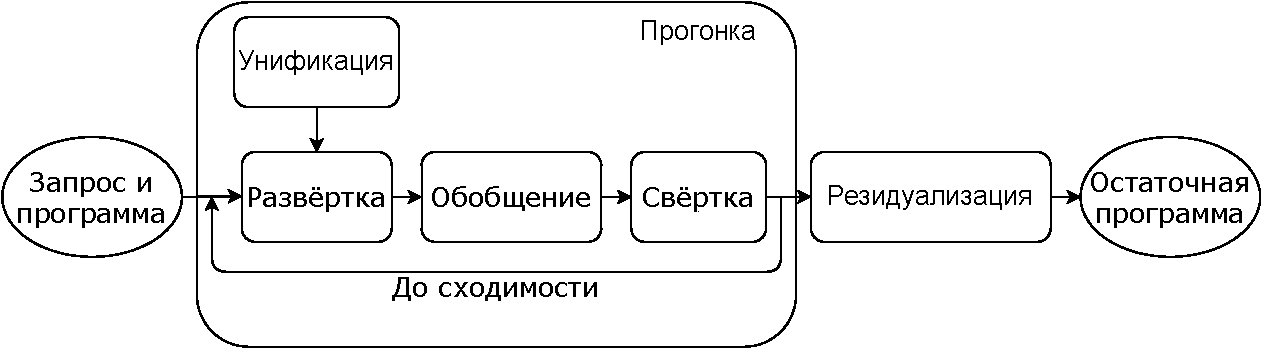
\includegraphics[width=\textwidth]{Kuklina/src/review/scompflow.pdf}
\caption{Общая схема суперкомпилятора.}
\label{fig:scompScheme}
\end{figure}

История вычислений при суперкомпиляции представляется в виде \emph{графа процессов} --- корневого ориентированного графа,
в котором каждая ветвь --- это отдельный путь вычислений, а каждый узел --- состояние системы или \emph{конфигурация}.
Конфигурация обобщённо описывает множество состояний вычислительной системы или её подсистемы.
К примеру, конфигурацией можно назвать выражение $1 + x$, в котором параметр $x$ пробегает
все возможные значения своего домена (допустим, множество натуральных чисел) и задаёт
таким образом множество состояний программы~\cite{turchinSC}.

% Процесс построения графа процессов называется \emph{прогонкой} \origin{driving}.
\emph{Прогонкой}~\origin{driving} называется процесс построения графа процессов.
Во время прогонки производится шаг символьных вычислений, после которого
в граф процессов добавляются порождённые конфигурации; множество конфигураций
появляется тогда, когда ветвления в программе зависят от свободных переменных.
В данной работе шаг символьного вычисления именуется \emph{развёрткой}.

В процессе прогонки в конфигурациях могут появляться новые свободные переменные,
которые строятся из исходной конфигурации:
если при вычислении выражения его переменная перешла в другую переменную (к примеру, из-за сопоставления с образцом),
то в итоговую конфигурацию будет подставлена новая переменная и связь старой и новой сохранится в
некоторой \emph{подстановке}.
Подстановка --- это отображение из множества переменных в множество возможно замкнутых термов.
Применение подстановки к выражению заменит все вхождения переменных, принадлежащих её домену,
на соответствующие термы. %\todo{Что-нибудь ещё}

Пример графа процессов представлен на рисунке~\ref{fig:pgraphExample}.
\begin{figure}[h!]
\center
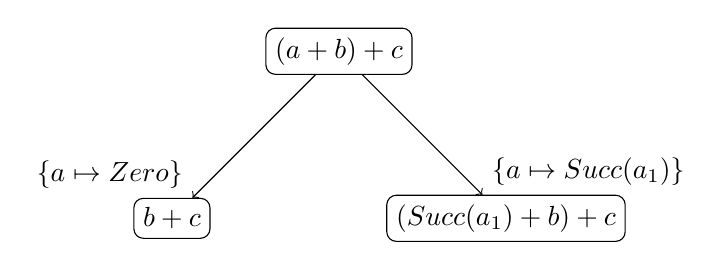
\begin{tikzpicture}[->,node distance=3cm, sibling distance=5cm]

  \tikzstyle{conf}=[rectangle,draw, rounded corners=.8ex]

  \node[conf] (root) {$(a + b) + c$} ;
  \node[conf] (childLeft) [below left of = root] {$b + c$};
  \node[conf] (childRight)[below right of = root] {$(\text{Succ}(a_1) + b) + c$};
  \path (root) edge node[above left,pos=1] {$\{a \mapsto \text{Zero}\}$} (childLeft)
        (root) edge node[above right,pos=1]{$\{a \mapsto \text{Succ}(a_1)\}$}(childRight);
\end{tikzpicture}

\caption{Пример части графа процессов.}
\label{fig:pgraphExample}
\end{figure}
Здесь при исполнении выражения $(a + b) + c$, где $a, b, c$ -- натуральные числа,
были рассмотрены возможные значения $a$: либо оно равно нулю (конструктор Zero), либо это некоторое
число $a_1$, которому прибавили единицу (конструктор Succ). Эти два случая могут задавать
различные пути исполнения и, соответственно, добавлены в дерево процессов как два различных состояния,
в одно из которых войдёт программа при исполнении.

Процесс прогонки может быть бесконечным, к примеру, когда происходят рекурсивные вызовы.
Для превращения бесконечного дерева вычисления в конечный объект, по которому можно
восстановить исходное дерево, используется \emph{свёртка.}

Свёртка~\origin{folding}~--- это процесс преобразования дерева процессов в граф, при котором
из вершины $v_c$ добавляется ребро в родительскую вершину $v_p$,
если выражение в конфигурации в $v_c$ и в $v_p$ равны с точностью до переименования.
Пример ситуации для свёртки изображён на рисунке~\ref{fig:pgraphFoldingExample},
на котором свёрточное ребро изображено пунктиром.

\begin{figure}[h!]
\center
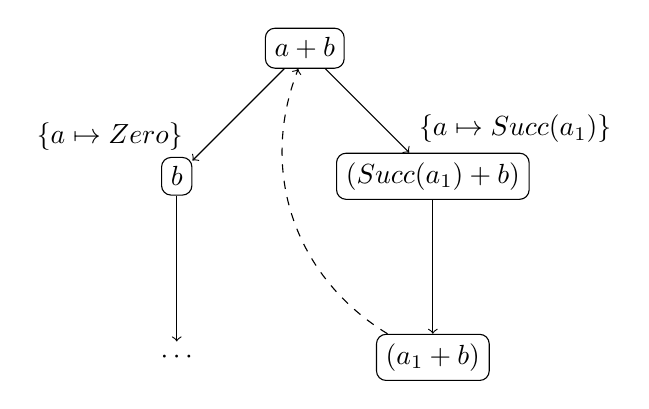
\begin{tikzpicture}[->,node distance=2.3cm, sibling distance=5cm]

  \tikzstyle{conf}=[rectangle,draw, rounded corners=.8ex]

  \node[conf] (root) {$a + b$} ;
  \node[conf] (childLeft) [below left of = root] {$b$};
  \node[conf] (childRight)[below right of = root] {$(\text{Succ}(a_1) + b)$};
  \node[conf] (childRight2)[below  of = childRight] {$(a_1 + b)$};
  \node (left)[below of = childLeft] {$\cdots$};

  \path (root) edge node[above left,pos=1] {$\{a \mapsto \text{Zero}\}$} (childLeft)
        (root) edge node[above right,pos=1]{$\{a \mapsto \text{Succ}(a_1)\}$}(childRight)
        (childLeft) edge (left)
        (childRight) edge (childRight2)
        (childRight2) edge[bend left=40, dashed] (root);
  %\draw[->] (childRight) to (childRight2);
  %\draw[->,dashed] (childRight2) to[bend left=90] (root);
\end{tikzpicture}

\caption{Пример свёртки.}
\label{fig:pgraphFoldingExample}
\end{figure}

Однако существуют ситуации, при которых свёртка не приведёт к тому, что граф превратится в
конечный объект. Такое может произойти, к примеру, когда два выражения структурно
схожи, но не существует переименования, уравнивающих их.

Для решения этой проблемы используется \emph{обобщение}~\cite{scGen}. Обобщение --- это процесс
замены одной конфигурации на другую, более абстрактную, описывающую больше состояний
программы. Для обнаружения ``похожей'' конфигурации используется предикат,
традиционно называемый \emph{свистком}:
% свисток пробегает по всем родителям текущей конфигурации и
свисток определяет, похожа ли конфигурация на кого-то из родителей текущей конфигурации.
В случае, когда свисток сигнализирует о найденной схожести, применяется обобщение.
Сам шаг обобщения может произвести действия двух видов:
\begin{itemize}
\item \emph{обобщение вниз} приводит к тому, что новая конфигурация заменяет текущую в графе процессов;
%\item \emph{обобщение вверх} приводит к замене родительской конфигурации на обобщённую;
\item \emph{разделение}~\origin{split} используется для декомпозиции выражения, элементы которого затем
будут обработаны отдельно.
\end{itemize}
Пример обобщения представлен на рисунке~\ref{fig:pgraphGenExample}
\begin{figure}[h!]
  \centering
  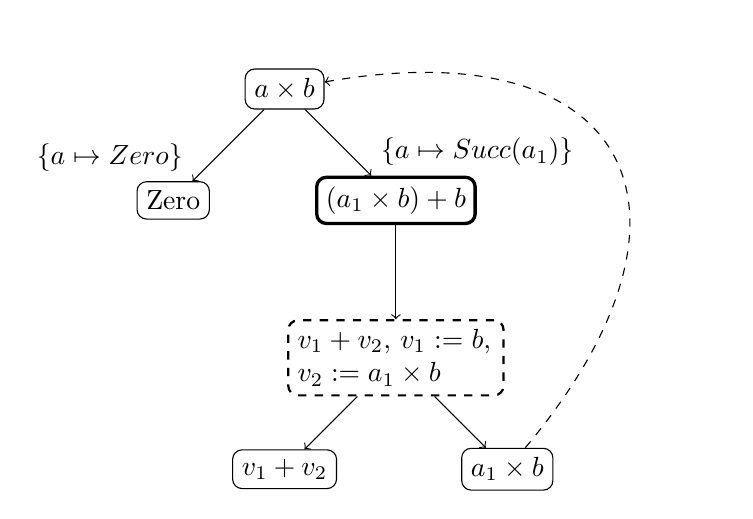
\begin{tikzpicture}[->,node distance=2cm, sibling distance=5cm]
    \tikzstyle{conf}=[rectangle,draw, rounded corners=.8ex]
    \node[conf] (root) {$a \times b$};
    \node[conf] (childLeft)[below left of = root] {Zero};
    \node[conf, very thick] (childRight)[below right of = root] {$(a_1 \times b) + b$};
    \node[conf, text width = 2.5cm, thick, dashed] (childGen)[below of = childRight] {$v_1 + v_2$, $v_1 := b$, $v_2 := a_1 \times b$};
    \node[conf] (childGenLeft)[below left of = childGen] {$v_1 + v_2$};
    \node[conf] (childGenRight)[below right of = childGen] {$a_1 \times b$};

    \path (root) edge node[above left,pos=1] {$\{a \mapsto \text{Zero}\}$} (childLeft)
          (root) edge node[above right,pos=1]{$\{a \mapsto \text{Succ}(a_1)\}$}(childRight)
          (childRight) edge (childGen)
          (childGen) edge (childGenLeft)
          (childGen) edge (childGenRight)
    ;

    \draw[->, dashed] (childGenRight) to[out=50,in=10,looseness=1.9] (root);
  \end{tikzpicture}
\caption{Пример обобщения.}
\label{fig:pgraphGenExample}
\end{figure}

Построение программы по графу конфигураций называется \emph{резидуализацией}, а
построенная программа --- \emph{остаточной} \origin{residual}.
Алгоритм выявления остаточной программы основан на обходе дерева, но
в остальном полностью зависит от языка.



\subsection{Постановка задачи}

Таким образом, целью данной работы является улучшение качества специализации
реляционных программ на miniKanren с использованием методов суперкомпиляции.
Для этого были поставлены следующие задачи:
\begin{itemize}
\item реализовать базовый суперкомпилятор;
\item рассмотреть и реализовать возможные модификации алгоритма суперкомпиляции,
      учитывающие свойства реляционных языков;
\item произвести экспериментальное исследование результата.
\end{itemize}
